%To perform proper speech recognition, knowing the direction of the sound is important to capture the sound source properly.
We localize the sound source by determining the \acrfull{doa} using a Matrix Creator\footnote{\url{https://creator.matrix.one}} board.
%depicted in Figure \ref{fig:matrix_one}.
%\begin{figure}[h]
%    \centering
%    %\vspace{-0.3cm}
%	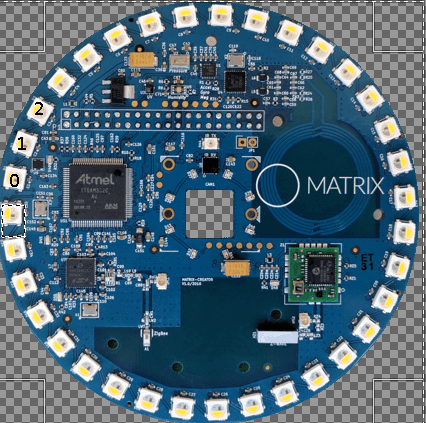
\includegraphics[width = 0.5\linewidth]{Figures/ssl_Matrix_creator.png}
%    %\vspace{-1em}
%	\caption{Matrix One Creator board.}
%	\label{fig:matrix_one}
%    %\vspace{-0.5cm}
%\end{figure}
%The detection is done by first calculating the time cross correlation between four pairs of opposing microphones.
%Second, the microphone pair with the lowest phase shift w.r.t. the opposing microphone is selected as being perpendicular to the source.
%Finally, the direction of the source can be determined by combining this information with the energy level of the microphones.
The detection is done by cross-correlating between pairs of opposing microphone, combined with finding the two microphones with the lowest mutual phase shift and using the energy level of the microphones.
%This upgrade compared to the stock DOA code of the Matrix Creator has been pushed back to their repositories.
This improvement is contributed back into the upstream repository.
%Our software for the DOA detection is available on GitHub\footnote{\url{https://github.com/tue-robotics/matrix-creator-hal}}, as well as a ROS package\footnote{\url{https://github.com/tue-robotics/matrix_creator_ros}} that exposes the DOA detections via a pose topic.
The \acrshort{doa} is published as a ROS Pose. Because the DSPL doesn't allow hardware changes to the robot, this software needs to be re-implemented for the Toyota HSR.

